% !TeX root = hack-the-universe.tex
% !TeX TXS-program:compile = txs:///pdflatex/[--shell-escape]
% !TeX encoding = UTF-8
% !TeX spellcheck = en_US
% https://orcid.org/0000-0003-4586-8500

%\documentclass[14pt]{beamer}
\documentclass[aspectratio=169]{beamer} % Other possible values are: 1610, 149, 54, 43 and 32. By default, it is to 128mm by 96mm(4:3)

\usepackage[utf8]{inputenc}
\usepackage[T1]{fontenc}
\usepackage{graphicx}

\usepackage{helvet}
\renewcommand{\familydefault}{\sfdefault}

% no navigation symbols
\setbeamertemplate{navigation symbols}{}

% Text positioning
\usepackage[absolute,overlay]{textpos}

% https://hartwork.org/beamer-theme-matrix/
\definecolor{bulletcolor}{RGB}{0,0,0} % RGB model is defined with values between 0 and 255
\setbeamercolor{local structure}{fg=bulletcolor}
\setbeamertemplate{itemize items}[circle]

% make the hyperlinks blue
\usepackage{hyperref}
\hypersetup{colorlinks=true,urlcolor=blue}

\usepackage{physics}

%\usepackage{biblatex}



\begin{document}

\usebackgroundtemplate{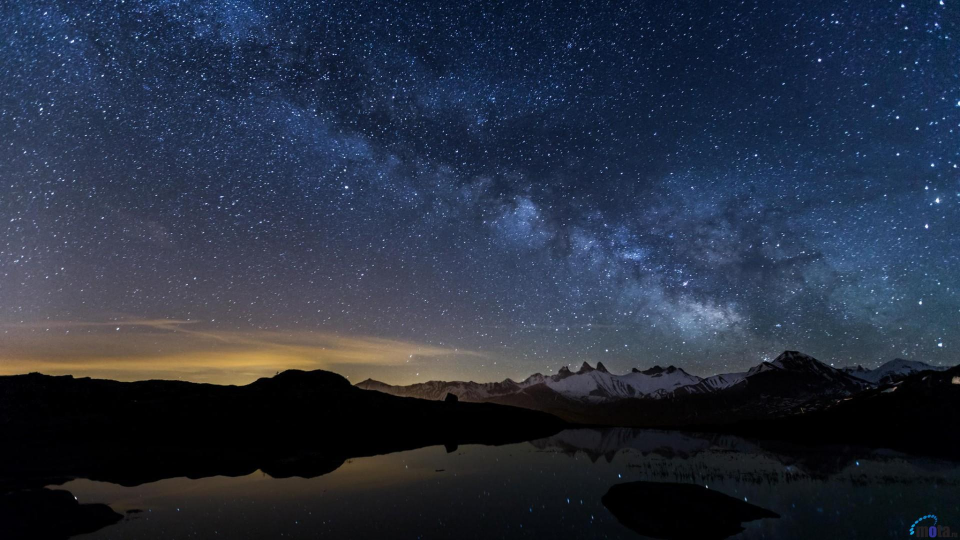
\includegraphics[width=\paperwidth]{../images/background.png}}
\begin{frame}{}
    \setlength{\TPHorizModule}{\textwidth}
    \setlength{\TPVertModule}{\textwidth}
    % Slide title in upper left
    \begin{textblock}{0.74}(0.30,0.25)
        \bfseries\huge\textcolor{yellow}{HACK THE UNIVERSE}
    \end{textblock}
    \begin{textblock}{0.74}(0.40,0.35)
    \bfseries\large\textcolor{yellow}{Amateur Radio Astronomy}
\end{textblock}
\end{frame}

\usebackgroundtemplate{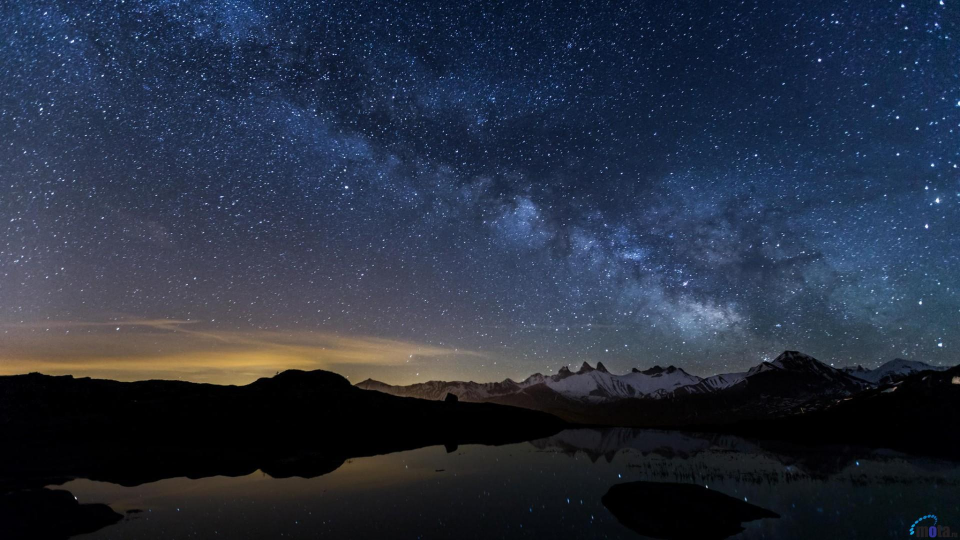
\includegraphics[width=\paperwidth]{../images/background.png}}
\begin{frame}{}
    \setlength{\TPHorizModule}{\textwidth}
    \setlength{\TPVertModule}{\textwidth}
    % Slide title in upper left
    \begin{textblock}{0.74}(0.05,0.05)
        \bfseries\huge\textcolor{yellow}{DISCLAIMER}
    \end{textblock}

    \begin{flushright}
    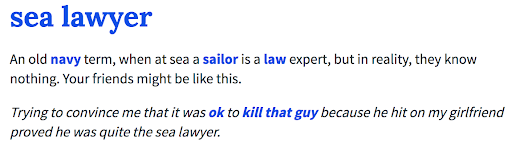
\includegraphics[width=0.65\linewidth, height=0.3\textheight]{../images/sea_lawyer.png}
    \end{flushright}

    \begin{itemize}
        \color{yellow}
        \item I am not a physicist, cosmologist, chemist or other field related to RA.
        \item My work experience and degrees are all computer network/security related.
        \item My interest and experience with RA are purely amateur/hobby related
        \item Committed to a life of understanding to the extent possible
        \item I do misspeak and make mistakes, there are many things I don’t know (but want to)
        \item The onus for discretionary use of the information presented herein is your responsibility
        \item Also I’m not a lawyer, so this disclaimer is invalid
    \end{itemize}


\end{frame}

\usebackgroundtemplate{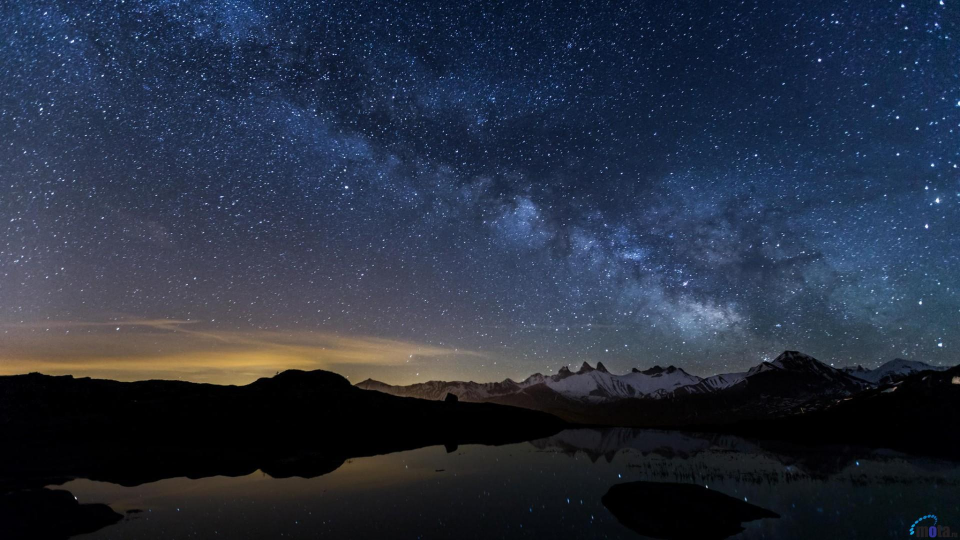
\includegraphics[width=\paperwidth]{../images/background.png}}
\begin{frame}{}
    \setlength{\TPHorizModule}{\textwidth}
    \setlength{\TPVertModule}{\textwidth}
    % Slide title in upper left
    \begin{textblock}{0.74}(0.25,0.35)
        \bfseries\huge\textcolor{yellow}{Some Introductory Concepts}
    \end{textblock}
\end{frame}

\usebackgroundtemplate{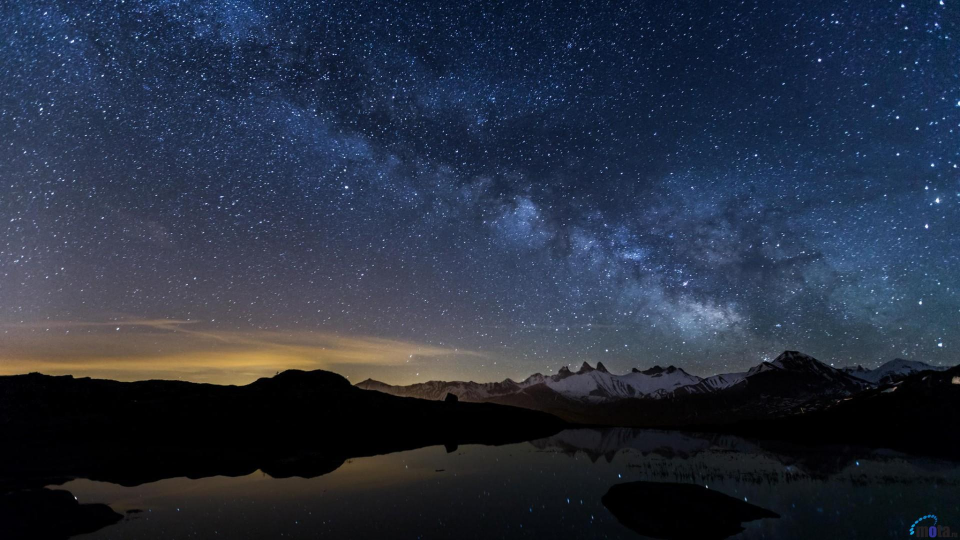
\includegraphics[width=\paperwidth]{../images/background.png}}
\begin{frame}{}
    \setlength{\TPHorizModule}{\textwidth}
    \setlength{\TPVertModule}{\textwidth}
    % Slide title in upper left
    \begin{textblock}{0.74}(0.05,0.04)
        \bfseries\huge\textcolor{yellow}{What is Radio Astronomy}
    \end{textblock}
    \begin{columns}
    \begin{column}{0.6\textwidth}

    \begin{itemize}
    \color{yellow}
        \item Radio astronomy is the study of celestial objects that give off radio waves.
        \item With radio astronomy, we study astronomical phenomena that are often invisible or hidden in other portions of the electromagnetic spectrum.
        \item Want to make the distinction between optical and radio astronomy.
        \item Optical Astronomy has been around as long as people have been looking at the night sky.
            \begin{itemize}
            \color{yellow}
        \item RA is much newer
        \item RA is very technology driven.
     \end{itemize}\end{itemize}

        \end{column}
\begin{column}{0.35\textwidth}
\begin{center}
    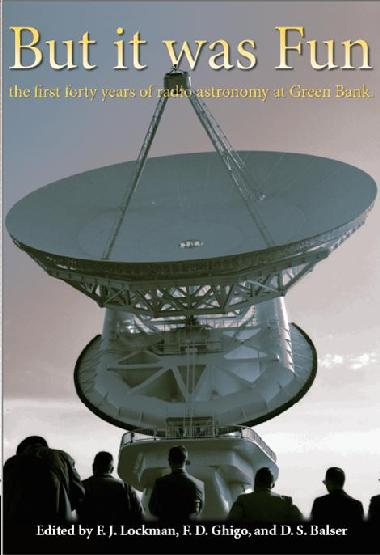
\includegraphics[width=1.0\linewidth, height=0.85\textheight]{../images/but_it_was_fun_cover.jpeg}
\end{center}
\end{column}
\end{columns}


\end{frame}

\end{document}